% Generated by tools/export_latex.go. Do not edit.
% Per-image phase breakdown of one evaluation pass (pgfplots); Tier 3 is bounded below by the probe window
% Source: empirical_study.json sha256 8bedcdc8173311ca7e44e464223f9d39bd2332b79fd475eec7ef0f5701cc0e50
% Images are chosen at evenly spaced ranks of total duration.
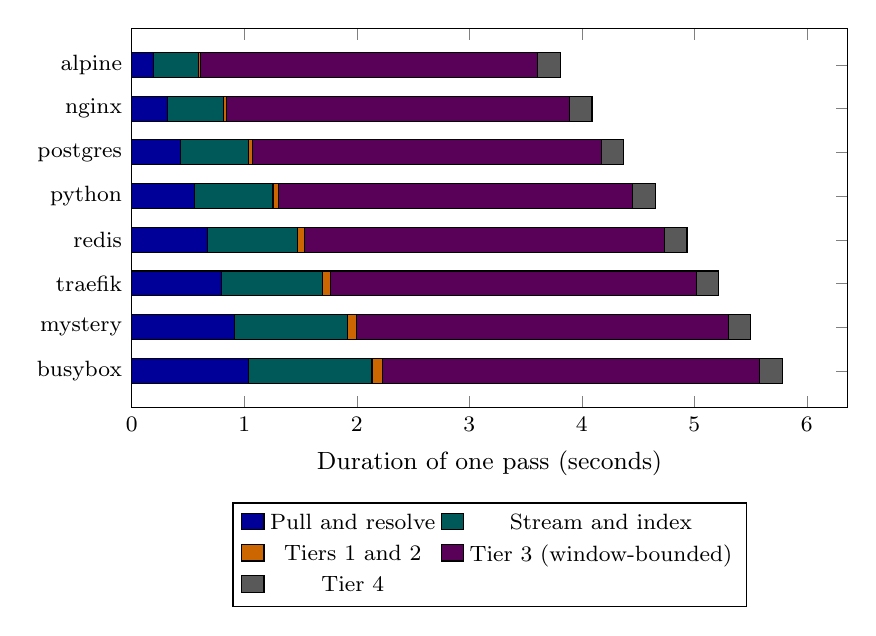
\begin{tikzpicture}
\begin{axis}[
    xbar stacked,
    width=0.88\columnwidth,
    height=6.4cm,
    xlabel={Duration of one pass (seconds)},
    symbolic y coords={alpine,nginx,postgres,python,redis,traefik,mystery,busybox},
    ytick=data,
    xmin=0,
    enlarge y limits=0.12,
    bar width=9pt,
    y dir=reverse,
    legend style={at={(0.5,-0.25)}, anchor=north, legend columns=2, font=\footnotesize},
    tick label style={font=\footnotesize},
    label style={font=\small},
]
\addplot[fill=blue!60!black] coordinates {
    (0.195,alpine)
    (0.315,nginx)
    (0.435,postgres)
    (0.555,python)
    (0.675,redis)
    (0.795,traefik)
    (0.915,mystery)
    (1.035,busybox)
};
\addlegendentry{Pull and resolve}
\addplot[fill=teal!70!black] coordinates {
    (0.400,alpine)
    (0.500,nginx)
    (0.600,postgres)
    (0.700,python)
    (0.800,redis)
    (0.900,traefik)
    (1.000,mystery)
    (1.100,busybox)
};
\addlegendentry{Stream and index}
\addplot[fill=orange!80!black] coordinates {
    (0.013,alpine)
    (0.025,nginx)
    (0.036,postgres)
    (0.049,python)
    (0.060,redis)
    (0.072,traefik)
    (0.085,mystery)
    (0.097,busybox)
};
\addlegendentry{Tiers 1 and 2}
\addplot[fill=violet!70!black] coordinates {
    (3.000,alpine)
    (3.050,nginx)
    (3.100,postgres)
    (3.150,python)
    (3.200,redis)
    (3.250,traefik)
    (3.300,mystery)
    (3.350,busybox)
};
\addlegendentry{Tier 3 (window-bounded)}
\addplot[fill=gray!70!black] coordinates {
    (0.200,alpine)
    (0.200,nginx)
    (0.200,postgres)
    (0.200,python)
    (0.200,redis)
    (0.200,traefik)
    (0.200,mystery)
    (0.200,busybox)
};
\addlegendentry{Tier 4}
\end{axis}
\end{tikzpicture}
